%%
%% This is file `sample-manuscript.tex',
%% generated with the docstrip utility.
%%
%% The original source files were:
%%
%% samples.dtx  (with options: `manuscript')
%% 
%% IMPORTANT NOTICE:
%% 
%% For the copyright see the source file.
%% 
%% Any modified versions of this file must be renamed
%% with new filenames distinct from sample-manuscript.tex.
%% 
%% For distribution of the original source see the terms
%% for copying and modification in the file samples.dtx.
%% 
%% This generated file may be distributed as long as the
%% original source files, as listed above, are part of the
%% same distribution. (The sources need not necessarily be
%% in the same archive or directory.)
%%
%% The first command in your LaTeX source must be the \documentclass command.
%%%% Small single column format, used for CIE, CSUR, DTRAP, JACM, JDIQ, JEA, JERIC, JETC, PACMCGIT, TAAS, TACCESS, TACO, TALG, TALLIP (formerly TALIP), TCPS, TDSCI, TEAC, TECS, TELO, THRI, TIIS, TIOT, TISSEC, TIST, TKDD, TMIS, TOCE, TOCHI, TOCL, TOCS, TOCT, TODAES, TODS, TOIS, TOIT, TOMACS, TOMM (formerly TOMCCAP), TOMPECS, TOMS, TOPC, TOPLAS, TOPS, TOS, TOSEM, TOSN, TQC, TRETS, TSAS, TSC, TSLP, TWEB.
% \documentclass[acmsmall]{acmart}

%%%% Large single column format, used for IMWUT, JOCCH, PACMPL, POMACS, TAP, PACMHCI
% \documentclass[acmlarge,screen]{acmart}

%%%% Large double column format, used for TOG
% \documentclass[acmtog, authorversion]{acmart}

%%%% Generic manuscript mode, required for submission
%%%% and peer review
\documentclass[manuscript,screen,review]{acmart}
%% Fonts used in the template cannot be substituted; margin 
%% adjustments are not allowed.
%%
%% \BibTeX command to typeset BibTeX logo in the docs
\AtBeginDocument{%
  \providecommand\BibTeX{{%
    \normalfont B\kern-0.5em{\scshape i\kern-0.25em b}\kern-0.8em\TeX}}}

%% Rights management information.  This information is sent to you
%% when you complete the rights form.  These commands have SAMPLE
%% values in them; it is your responsibility as an author to replace
%% the commands and values with those provided to you when you
%% complete the rights form.
\setcopyright{acmcopyright}
\copyrightyear{2018}
\acmYear{2018}
\acmDOI{10.1145/1122445.1122456}

%% These commands are for a PROCEEDINGS abstract or paper.
\acmConference[Woodstock '18]{Woodstock '18: ACM Symposium on Neural
  Gaze Detection}{June 03--05, 2018}{Woodstock, NY}
\acmBooktitle{Woodstock '18: ACM Symposium on Neural Gaze Detection,
  June 03--05, 2018, Woodstock, NY}
\acmPrice{15.00}
\acmISBN{978-1-4503-XXXX-X/18/06}


%%
%% Submission ID.
%% Use this when submitting an article to a sponsored event. You'll
%% receive a unique submission ID from the organizers
%% of the event, and this ID should be used as the parameter to this command.
%%\acmSubmissionID{123-A56-BU3}

%%
%% The majority of ACM publications use numbered citations and
%% references.  The command \citestyle{authoryear} switches to the
%% "author year" style.
%%
%% If you are preparing content for an event
%% sponsored by ACM SIGGRAPH, you must use the "author year" style of
%% citations and references.
%% Uncommenting
%% the next command will enable that style.
%%\citestyle{acmauthoryear}

%%
%% end of the preamble, start of the body of the document source.
\begin{document}

%%
%% The "title" command has an optional parameter,
%% allowing the author to define a "short title" to be used in page headers.
\title{Neuroadaptive Haptics: Probing Brain Signals to Optimize Perceived Haptics}

%%
%% The "author" command and its associated commands are used to define
%% the authors and their affiliations.
%% Of note is the shared affiliation of the first two authors, and the
%% "authornote" and "authornotemark" commands
%% used to denote shared contribution to the research.
\author{Lukas Gehrke}
% \authornote{Both authors contributed equally to this research.}
\email{lukas-gehrke@tu-berlin.de}
\orcid{1234-5678-9012}
\affiliation{%
  \institution{TU Berlin}
  \streetaddress{Straße des 17. Juni 135}
  \city{Berlin}
  \state{Berlin}
  \country{Germany}
  \postcode{10623}
}

%%
%% By default, the full list of authors will be used in the page
%% headers. Often, this list is too long, and will overlap
%% other information printed in the page headers. This command allows
%% the author to define a more concise list
%% of authors' names for this purpose.
\renewcommand{\shortauthors}{Gehrke et al.}

%%
%% The abstract is a short summary of the work to be presented in the
%% article.
\begin{abstract}
  
% Besides the title, this is what most people (90+%) will read from your paper!

% - [ ] Therefore, improve SEO (Search engine optimization): copy the abstract text to hemingwayapp.com to improve information density, keyword frequency and readability! Go through each sentence to shorten it and remove unnecessary words.

abstract text there only


\end{abstract}

%%
%% The code below is generated by the tool at http://dl.acm.org/ccs.cfm.
%% Please copy and paste the code instead of the example below.
%%
\begin{CCSXML}
<ccs2012>
 <concept>
  <concept_id>10010520.10010553.10010562</concept_id>
  <concept_desc>Computer systems organization~Embedded systems</concept_desc>
  <concept_significance>500</concept_significance>
 </concept>
 <concept>
  <concept_id>10010520.10010575.10010755</concept_id>
  <concept_desc>Computer systems organization~Redundancy</concept_desc>
  <concept_significance>300</concept_significance>
 </concept>
 <concept>
  <concept_id>10010520.10010553.10010554</concept_id>
  <concept_desc>Computer systems organization~Robotics</concept_desc>
  <concept_significance>100</concept_significance>
 </concept>
 <concept>
  <concept_id>10003033.10003083.10003095</concept_id>
  <concept_desc>Networks~Network reliability</concept_desc>
  <concept_significance>100</concept_significance>
 </concept>
</ccs2012>
\end{CCSXML}

\ccsdesc[500]{Computer systems organization~Embedded systems}
\ccsdesc[300]{Computer systems organization~Redundancy}
\ccsdesc{Computer systems organization~Robotics}
\ccsdesc[100]{Networks~Network reliability}

%%
%% Keywords. The author(s) should pick words that accurately describe
%% the work being presented. Separate the keywords with commas.
\keywords{datasets, neural networks, gaze detection, text tagging}

%% A "teaser" image appears between the author and affiliation
%% information and the body of the document, and typically spans the
%% page.

% This is what most people (90+%) will see from your paper!

% - [ ]  use hemingwayapp.com (+SEO if hardcore) to make figure captions super precise
% - [ ]  are all the axes labels readable, font size 10 or up
% - [ ]  check for missing information: give someone the figure with captions to someone neutral to check if everything is clear from the figure alone
% - [ ]  for digital version: what is alt-text of figure, i.e. when hovering with the mouse over the figure what text appears next to the cursor
% - [ ]  for accessibility: write figure caption for the blind
%     - [ ]  explain what the figure shows
%     - [ ]  refactor using hemingwayapp.com

\begin{teaserfigure}
  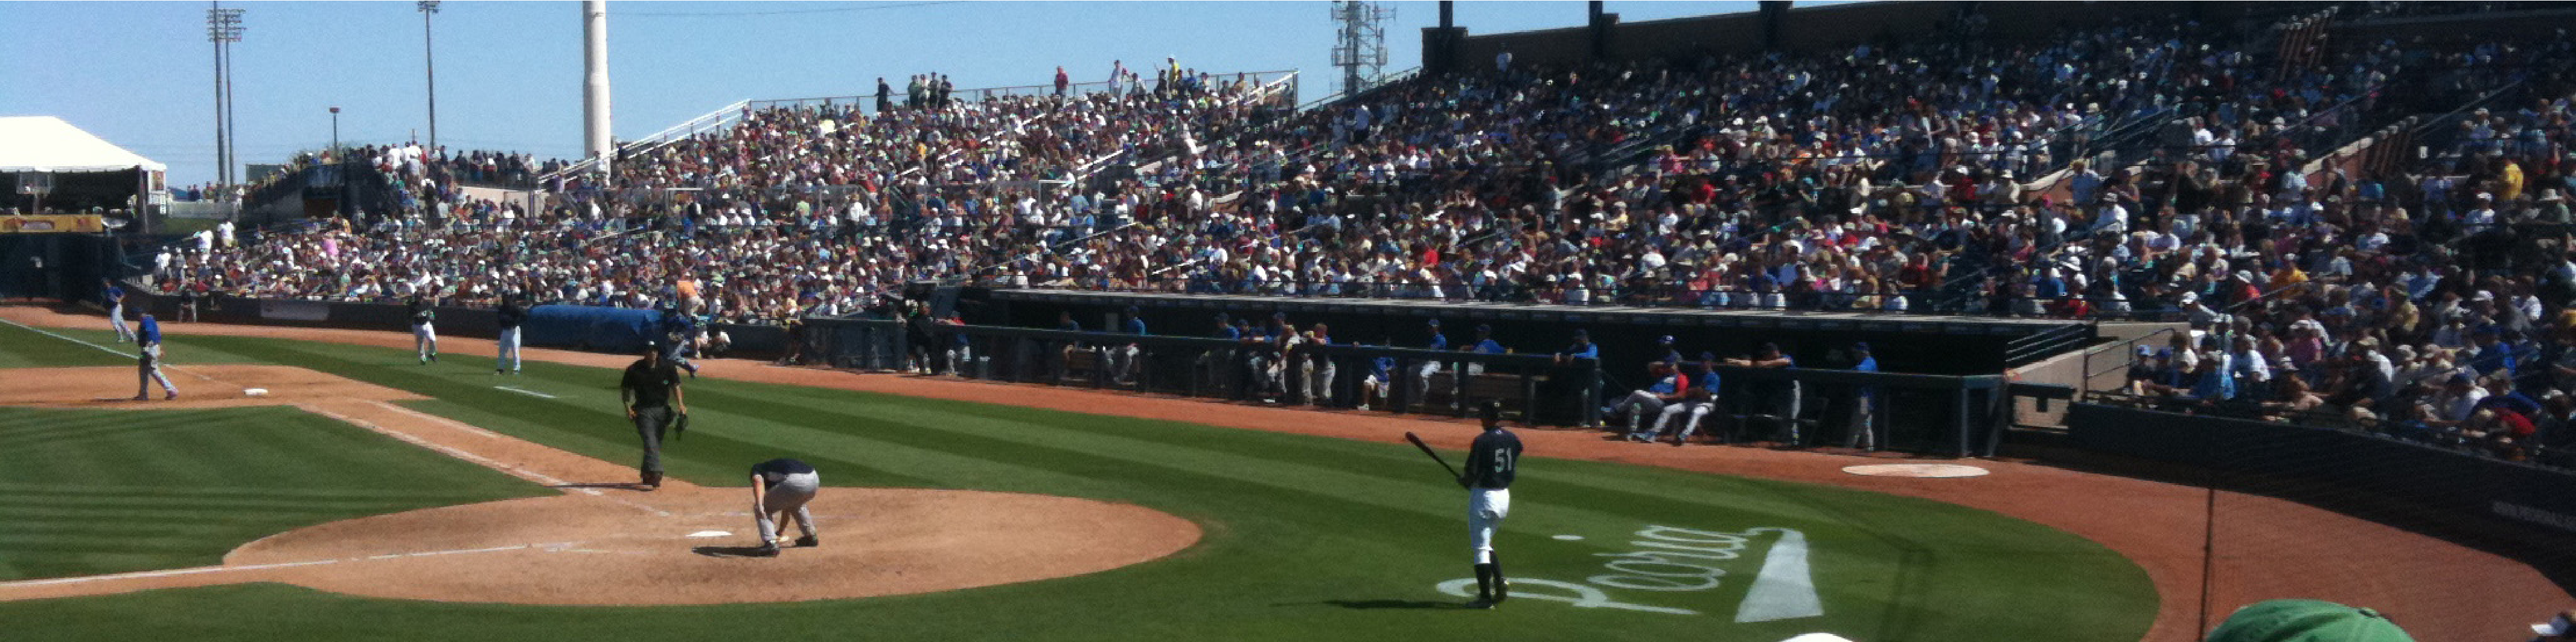
\includegraphics[width=\textwidth]{tex_sample_files/sampleteaser.pdf}
  \caption{Seattle Mariners at Spring Training, 2010.}
  \Description{Enjoying the baseball game from the third-base
  seats. Ichiro Suzuki preparing to bat.}
  \label{fig:teaser}
\end{teaserfigure}

%%
%% This command processes the author and affiliation and title
%% information and builds the first part of the formatted document.
\maketitle

\section{Introduction}
% Lukas note:
% I like to use SCQA (Situation, Complication, Question, Answer) 'system' to write the introduction, see one of the two links below
% https://analytic-storytelling.com/scqa-what-is-it-how-does-it-work-and-how-can-it-help-me/
% https://corporatefinanceinstitute.com/resources/careers/how-to-job-guides/scqa/
% https://karrierebibel.de/scqa-methode/

% 1. Describe the Current Situtation
% Functions as a starting point and a common basis. Therefore it primarily contains recognizable and agreed points.

% 2. What is the complication, challenge identified
% Spells the reason for acting now. It contains threats / opportunities and the hurdles that need to be overcome.

% 3. Question
% Asks the question how the hurdles of the Complication can be overcome. How can we prevent the threat or seize the opportunity? Also, what would be the benefits if the complication would be overcome?

% 4. (short) Answer Teaser
% Provides the answer on how to overcome the hurdles. Explains how this will help deflect the threats or seize the opportunities.
% keep this short

\subsection{Main contribution: Our proposed solution}
% 4. (long) Anwser with teaser image
% Provides the answer on how to overcome the hurdles. Explains how this will help deflect the threats or seize the opportunities.
% Now extend into a longer paragraph with a teaser image explaining the system in the following subsection

% for citations use use "~\cite{}" instead of " \cite{}" → no white space, copy bibtex items to cite into input/bibliography.bib
% example:
some text~\cite{Gehrke2019-og}


% This is what most people (90+%) will see from your paper!

% - [ ]  use hemingwayapp.com (+SEO if hardcore) to make figure captions super precise
% - [ ]  are all the axes labels readable, font size 10 or up
% - [ ]  check for missing information: give someone the figure with captions to someone neutral to check if everything is clear from the figure alone
% - [ ]  for digital version: what is alt-text of figure, i.e. when hovering with the mouse over the figure what text appears next to the cursor
% - [ ]  for accessibility: write figure caption for the blind
%     - [ ]  explain what the figure shows
%     - [ ]  refactor using hemingwayapp.com

\begin{teaserfigure}
  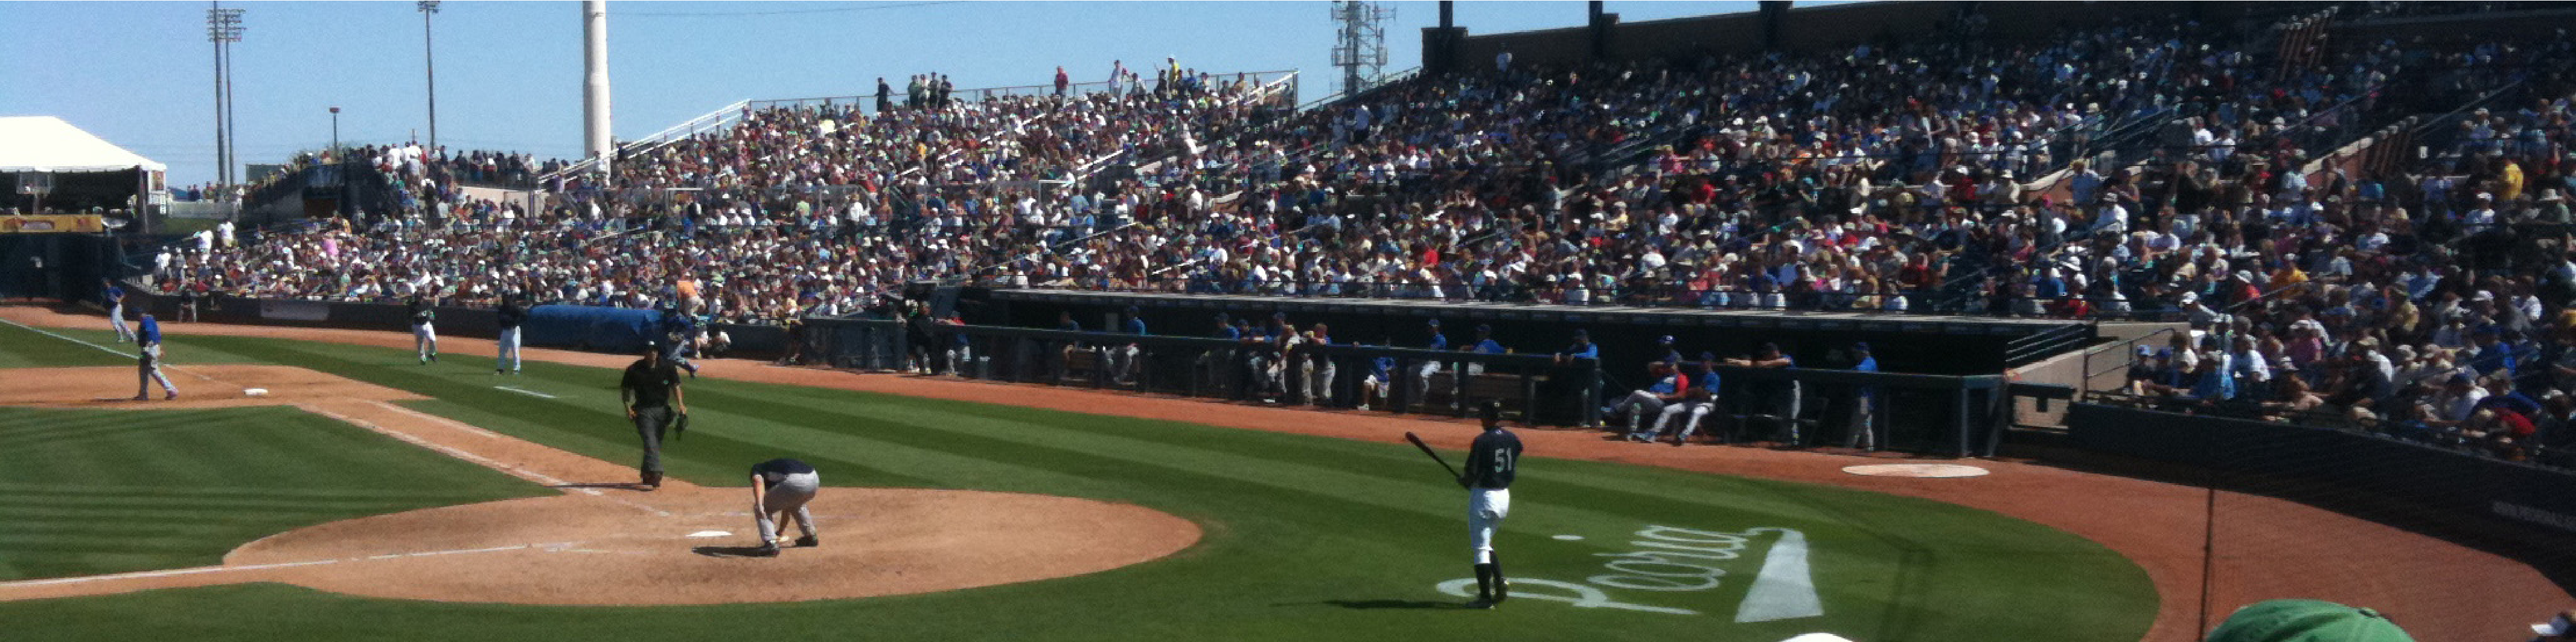
\includegraphics[width=\textwidth]{tex_sample_files/sampleteaser.pdf}
  \caption{Seattle Mariners at Spring Training, 2010.}
  \Description{Enjoying the baseball game from the third-base
  seats. Ichiro Suzuki preparing to bat.}
  \label{fig:teaser}
\end{teaserfigure}
\section{Related Work}

% Gender-inclusive: Relevant throughout the document but frequently occuring here:
% - [ ]  write gender-inclusive: do not use he or she but use they instead: "the participant was asking..., he liked ... → they liked (in singular)
% check for the following:
% - [ ]  Have you used “man” or “men” or words containing them to refer to people who may not be men?
% - [ ]  Have you used “he,” “him,” “his,” or “himself” to refer to people who may not be men?
% - [ ]  If you have mentioned someone’s sex or gender, was it necessary to do so?
% - [ ]  Do you use any occupational (or other) stereotypes?
% - [ ]  Do you provide the same kinds of information and descriptions when writing about people of different genders?

\section{User Study}

\section{Methods}
\section{Results}
\section{Discussion}
\section{Conclusions, Limitations and Opportunities}

%%
%% The acknowledgments section is defined using the "acks" environment
%% (and NOT an unnumbered section). This ensures the proper
%% identification of the section in the article metadata, and the
%% consistent spelling of the heading.
\begin{acks}

% no section, just write down the acknowledgements as text
\end{acks}

%%
%% The next two lines define the bibliography style to be used, and
%% the bibliography file.
\bibliographystyle{ACM-Reference-Format}
\bibliography{input/bibliography}

%%
%% If your work has an appendix, this is the place to put it.
\appendix


% appendix sections if necessary

\end{document}
\endinput
%%
%% End of file `sample-authordraft.tex'.
